% !TEX program = xelatex
\documentclass[10pt,a4paper]{article}

\usepackage[a4paper, top=19mm, bottom=21mm, left=19mm, right=19mm]{geometry}
\usepackage{fontspec}
\usepackage{xcolor}
\usepackage{graphicx}
\usepackage{booktabs}
\usepackage{tabularx}
\usepackage{xltabular}
\usepackage{colortbl}
\usepackage{array}
\usepackage{enumitem}
\usepackage{microtype}
\usepackage[most]{tcolorbox}
\usepackage{fancyhdr}
\usepackage{titlesec}
\usepackage{ragged2e}
\usepackage{setspace}
\usepackage{hyperref}
\usepackage{tikz}
\usetikzlibrary{arrows.meta, positioning, shapes.geometric, fit, backgrounds, calc}

\graphicspath{{figures/}}

% --- palette (muted, low-chroma editorial) ---------------------------------
% Role names are kept from SKILL.md so the body of the document is unchanged;
% only the values move. Chosen for a calm professional register rather than a
% saturated blue, and checked rather than eyeballed: crail 5.70:1 on white,
% coral 4.07:1, ink 14.54:1, inksoft 6.19:1 -- all clear their WCAG floors.
% The pale members (cream, creamline, coralwash, sagewash) are washes only and
% are never used for text or for a mark.
\definecolor{bluebase}{HTML}{35706B}
\definecolor{bluecyan}{HTML}{7FA9A3}
\definecolor{bluemid}{HTML}{4C8A83}
\definecolor{bluelight}{HTML}{A8C6C0}
\definecolor{bluewash}{HTML}{CFE0DC}
\definecolor{bluelink}{HTML}{35706B}
\definecolor{bluesoft}{HTML}{6E9C96}
\definecolor{bluedark}{HTML}{2C5F5A}

\definecolor{ivory}{HTML}{FBFCFB}
\definecolor{cream}{HTML}{EAF0EE}
\definecolor{creamline}{HTML}{DCE4E0}
\definecolor{ink}{HTML}{262A28}
\definecolor{inksoft}{HTML}{5B635E}
\definecolor{crail}{HTML}{35706B}
\definecolor{coral}{HTML}{A9705B}
\definecolor{coralwash}{HTML}{F5F1EC}
\definecolor{sagewash}{HTML}{EAF0EE}
\definecolor{sage}{HTML}{4C8A83}
\definecolor{rust}{HTML}{8F5C49}

\pagecolor{white}
\color{ink}

\hypersetup{
  colorlinks=true,
  linkcolor=crail,
  citecolor=crail,
  urlcolor=bluelink,
  linktoc=all,
  pdftitle={Bahdini QA Generation Pipeline},
  pdfauthor={Sawab Aziz}}

\setcounter{secnumdepth}{0}
\setcounter{tocdepth}{2}

% --- fonts -----------------------------------------------------------------
\IfFontExistsTF{Linux Libertine O}{
  \setmainfont{Linux Libertine O}[Ligatures=TeX, Numbers={Proportional,Lining}]
  \newfontfamily\headfont{Linux Libertine O}[Ligatures=TeX, Numbers={Proportional,Lining}]
}{
  \setmainfont{TeX Gyre Schola}[Ligatures=TeX, Numbers={Proportional,Lining}]
  \newfontfamily\headfont{TeX Gyre Schola}[Ligatures=TeX, Numbers={Proportional,Lining}]
}

\IfFontExistsTF{Poppins}{
  \newfontfamily\uifont{Poppins}[Ligatures=TeX]
  \newfontfamily\uimed{Poppins Medium}[Ligatures=TeX]
  \newfontfamily\uitrack{Poppins Medium}[Ligatures=TeX, LetterSpace=8.0]
  \newfontfamily\uitrackwide{Poppins Medium}[Ligatures=TeX, LetterSpace=14.0]
  \newfontfamily\uitracksm{Poppins Medium}[Ligatures=TeX, LetterSpace=4.0]
  \newfontfamily\uitrackmd{Poppins Medium}[Ligatures=TeX, LetterSpace=6.0]
}{
  \IfFontExistsTF{Inter}{
    \newfontfamily\uifont{Inter}[Ligatures=TeX]
    \newfontfamily\uimed{Inter}[Ligatures=TeX, UprightFont={* Medium}]
    \newfontfamily\uitrack{Inter}[Ligatures=TeX, UprightFont={* Medium}, LetterSpace=8.0]
    \newfontfamily\uitrackwide{Inter}[Ligatures=TeX, UprightFont={* Medium}, LetterSpace=14.0]
    \newfontfamily\uitracksm{Inter}[Ligatures=TeX, UprightFont={* Medium}, LetterSpace=4.0]
    \newfontfamily\uitrackmd{Inter}[Ligatures=TeX, UprightFont={* Medium}, LetterSpace=6.0]
  }{% Neither preferred UI face is installed. TeX Gyre Heros ships with every
   % TeX Live and MacTeX install, so this branch always resolves. Written out
   % literally rather than through a \def holding the family name: passing a
   % macro to \newfontfamily depends on expansion timing inside fontspec and
   % is not worth the risk in a document that must build unattended.
    \newfontfamily\uifont{TeX Gyre Heros}[Ligatures=TeX]
    \newfontfamily\uimed{TeX Gyre Heros}[Ligatures=TeX]
    \newfontfamily\uitrack{TeX Gyre Heros}[Ligatures=TeX, LetterSpace=8.0]
    \newfontfamily\uitrackwide{TeX Gyre Heros}[Ligatures=TeX, LetterSpace=14.0]
    \newfontfamily\uitracksm{TeX Gyre Heros}[Ligatures=TeX, LetterSpace=4.0]
    \newfontfamily\uitrackmd{TeX Gyre Heros}[Ligatures=TeX, LetterSpace=6.0]
  }
}

% Every fallback chain below ends in a face that ships inside TeX Live itself,
% not one that merely happens to be on this Mac. That is what lets the same
% source build unchanged on Overleaf's Linux containers, where Menlo and
% Geeza Pro do not exist and \setmonofont on a missing font is a hard error.
\IfFontExistsTF{DejaVu Sans Mono}{\setmonofont{DejaVu Sans Mono}[Scale=0.84]}{
  \IfFontExistsTF{Menlo}{\setmonofont{Menlo}[Scale=0.84]}
                        {\setmonofont{FreeMono}[Scale=0.84]}}

% Kurdish corpus excerpts. Noto Naskh Arabic is the intended face.
% Scheherazade New is the important fallback: it ships with TeX Live and
% covers the Kurdish-specific letters (ڤ ڕ ڵ ێ ۆ ە) that plainer Arabic faces
% often omit. Geeza Pro covers the macOS case, FreeSerif is the last resort
% and is always present in a full TeX Live.
\IfFontExistsTF{Noto Naskh Arabic}{
  \newfontfamily\kurdisharabicfont{Noto Naskh Arabic}[Script=Arabic, Scale=1.05]
}{
  \IfFontExistsTF{Scheherazade New}{
    \newfontfamily\kurdisharabicfont{Scheherazade New}[Script=Arabic, Scale=1.05]
  }{
    \IfFontExistsTF{Amiri}{
      \newfontfamily\kurdisharabicfont{Amiri}[Script=Arabic, Scale=1.05]
    }{
      \IfFontExistsTF{Geeza Pro}{
        \newfontfamily\kurdisharabicfont{Geeza Pro}[Script=Arabic, Scale=1.05]
      }{
        \newfontfamily\kurdisharabicfont{FreeSerif}[Script=Arabic, Scale=1.05]
      }
    }
  }
}
\IfFontExistsTF{DejaVu Sans}{\newfontfamily\corpuslatinfont{DejaVu Sans}[Scale=0.92]}
                            {\newfontfamily\corpuslatinfont{FreeSans}[Scale=0.92]}

% Right-to-left runs via XeTeX's own primitives rather than the bidi package.
% bidi must load last and is known to fight tcolorbox and tikz, both of which
% this document leans on heavily; the excerpts here are short, self-contained
% Arabic-script runs, which \beginR/\endR handles exactly.
\TeXXeTstate=1
\newcommand{\kurd}[1]{{\kurdisharabicfont\beginR #1\endR}}

\linespread{1.22}
\setlength{\parindent}{0pt}
\setlength{\parskip}{0.5em}
\emergencystretch=2em

\titleformat{\section}
  {\headfont\bfseries\fontsize{13.5}{17}\selectfont\color{crail}}
  {}{0pt}{}
\titlespacing*{\section}{0pt}{0.2em}{0.55em}

\titleformat{\subsection}
  {\headfont\bfseries\fontsize{11}{14}\selectfont\color{ink}}
  {}{0pt}{}
\titlespacing*{\subsection}{0pt}{0.85em}{0.2em}

\titleformat{\subsubsection}
  {\uitracksm\fontsize{8}{11}\selectfont\color{inksoft}\MakeUppercase}
  {}{0pt}{}
\titlespacing*{\subsubsection}{0pt}{0.2em}{0.35em}

\newtcolorbox{softcard}[1][]{
  enhanced, breakable,
  colback=cream!55!ivory, frame hidden,
  boxrule=0pt, arc=2.5mm,
  left=4mm, right=4mm, top=2.8mm, bottom=2.8mm,
  before skip=0.7em, after skip=0.7em, #1}

\newtcolorbox{warmcard}[1][]{
  enhanced, breakable,
  colback=coralwash!55!ivory, frame hidden,
  boxrule=0pt, arc=2.5mm,
  left=4mm, right=4mm, top=2.8mm, bottom=2.8mm,
  before skip=0.7em, after skip=0.7em, #1}

\newtcolorbox{sagecard}[1][]{
  enhanced, breakable,
  colback=sagewash!65!ivory, frame hidden,
  boxrule=0pt, arc=2.5mm,
  left=4mm, right=4mm, top=2.8mm, bottom=2.8mm,
  before skip=0.7em, after skip=0.7em, #1}

\newtcolorbox{corpuscard}[1][]{
  enhanced, breakable,
  colback=white, colframe=creamline,
  boxrule=0.45pt, arc=2.2mm,
  left=4mm, right=4mm, top=3mm, bottom=3mm,
  before skip=0.75em, after skip=0.9em, #1}

\newcommand{\chip}[1]{%
  {\uitracksm\fontsize{7.5}{9}\selectfont\color{crail}#1}\,\textcolor{creamline}{\rule[0.1ex]{0pt}{1ex}}}

\newcommand{\kw}[1]{\textbf{#1}}
\newcommand{\codeid}[1]{\texttt{\footnotesize\color{inksoft}#1}}
\newcommand{\corpusmeta}[2]{%
  {\uimed\fontsize{8}{10}\selectfont\color{crail}#1}\\[-0.1em]
  {\uifont\fontsize{7.5}{9.5}\selectfont\color{inksoft}#2}\par\vspace{0.45em}}

\newcommand{\preparedby}{%
  {\uifont\fontsize{8.5}{11}\selectfont\color{inksoft}%
  prepared by: \href{mailto:sawab.aziz@newrozholdings.com}{%
  \textcolor{bluelink}{\textbf{sawab.aziz@newrozholdings.com}}}}}

\tikzset{
  diagram node/.style={
    draw=creamline, fill=cream, rounded corners=2mm, line width=0.5pt,
    text=ink, align=center, inner xsep=3mm, inner ysep=2.2mm,
    font=\uifont\small},
  diagram accent/.style={diagram node, draw=crail, fill=coralwash},
  diagram arrow/.style={-{Latex[length=2.2mm]}, draw=crail, line width=0.65pt}}

\setlist[itemize]{
  label=\textcolor{inksoft}{\raisebox{0.28ex}{\scriptsize$\bullet$}},
  leftmargin=1.4em, itemsep=0.3em, topsep=0.25em, parsep=0pt}

\setlist[enumerate]{
  leftmargin=1.6em, itemsep=0.3em, topsep=0.25em, parsep=0pt,
  label={\bfseries\arabic*.}}

\newcolumntype{L}{>{\RaggedRight\arraybackslash}X}
\newcommand{\tablehead}[1]{{\uimed\fontsize{6.8}{8}\selectfont\color{crail}\mbox{#1}}}

\pagestyle{fancy}
\fancyhf{}
\renewcommand{\headrulewidth}{0pt}
\fancyhead[L]{\uitrackmd\fontsize{7.5}{9}\selectfont\color{inksoft}BAHDINI QA GENERATION}
\fancyhead[R]{\uifont\fontsize{7.5}{9}\selectfont\color{inksoft}Pipeline report, August 2026}
\fancyfoot[C]{\uifont\fontsize{8}{10}\selectfont\color{inksoft}\thepage}

\begin{document}

% ===========================================================================
\thispagestyle{empty}
\vspace*{6mm}

{\uitrackwide\fontsize{8}{10}\selectfont\color{crail}DATASET CONSTRUCTION REPORT}\\[5mm]
{\headfont\bfseries\fontsize{26}{31}\selectfont\color{ink}Bahdini Kurdish QA Generation}\\[4mm]
{\headfont\itshape\fontsize{12}{16}\selectfont\color{inksoft}How 246,515 text chunks became 952,801 instruction-tuning records, and what is wrong with them}\\[10mm]
{\uifont\fontsize{9}{13}\selectfont\color{inksoft}Corpus built 6--10 August 2026 \quad\textbullet\quad google/gemini-3.1-flash-lite \quad\textbullet\quad prompt v3 \quad\textbullet\quad \$301.41}\\[2mm]
\preparedby

\vspace{7mm}

\begin{softcard}
{\uimed\fontsize{8.5}{11}\selectfont\color{crail}WHAT THIS DOCUMENT IS}\par\vspace{0.3em}
This is the single source of truth for the QA-generation stage of the Bahdini
Kurdish fine-tuning corpus. It begins where the chunking stage ended --- with a
finished work queue of 246,515 text chunks --- and follows every step from
there to the delivered dataset, including the exact prompt sent to the model,
every token and dollar figure, the failure modes encountered, and the quality
problems that remain unresolved. Design decisions are recorded with the
reasoning behind them, so that a reader can tell which choices were forced,
which were measured, and which are still open to revision.
\end{softcard}

\vspace{2mm}
{\uitracksm\fontsize{8}{11}\selectfont\color{inksoft}CONTENTS}\par\vspace{-0.6em}
{\hypersetup{linkcolor=ink}
\renewcommand{\contentsname}{}
\vspace{-1.2em}
\tableofcontents}

\clearpage

% ===========================================================================
\section{At a glance}

\begin{softcard}
{\normalsize
\renewcommand{\arraystretch}{1.25}
\setlength{\tabcolsep}{4pt}
\begin{tabularx}{\textwidth}{@{}p{5.4cm}r@{\hspace{9mm}}p{4.6cm}r@{}}
\tablehead{INPUT} & & \tablehead{OUTPUT} & \\
\midrule
Chunks in the work queue & 246,515 & QA pairs generated & 952,822\\
Source documents & 4,306 & Records delivered & 952,801\\
Source corpora & 8 & Training tokens & 644,306,453\\
Context tokens in queue & 183,119,057 & Pairs with reasoning & 508,061\\
\end{tabularx}}

\vspace{1.5mm}
{\normalsize
\renewcommand{\arraystretch}{1.25}
\setlength{\tabcolsep}{4pt}
\begin{tabularx}{\textwidth}{@{}p{5.4cm}r@{\hspace{9mm}}p{4.6cm}r@{}}
\tablehead{API CONSUMPTION} & & \tablehead{COST} & \\
\midrule
Calls made & 248,243 & Total spend & \$301.41\\
Input tokens billed & 304,524,932 & Per 1,000 pairs & \$0.316\\
Output tokens billed & 150,188,299 & Per source chunk & \$0.00122\\
Total tokens billed & 454,713,231 & Cost-model error & 0.03\%\\
\end{tabularx}}
\end{softcard}

The two token totals in that table measure different things and are not
comparable. \kw{454.7M} is what the generation provider billed: the prompt sent
to Gemini plus the JSON it returned, counted by the provider's own tokenizer.
\kw{644.3M} is what the finished dataset contains: the assembled training
records counted with Gemma's tokenizer. The delivered corpus is larger than the
API traffic because each chunk's context is sent to the generator \emph{once}
but is then written into roughly three of the four training records built from
it.

% ===========================================================================
\section{Where this report begins}

The chunking stage is documented separately. This report takes its output as a
given and starts there, but three properties of that output determine
everything downstream and are restated here.

\subsection{What a chunk is}

A chunk is a contiguous passage of Bahdini text, packed paragraph-first to a
target of 900 real Gemma tokens with a hard ceiling of 1,050 and a floor of
120. The target was not chosen for the generator's convenience: the partner
specified a budget of roughly 1,000 tokens for the \emph{prompt side} of a
finished training record --- system message plus question plus context, with
the answer excluded --- expressed as a mean rather than a cap. Measuring the
fixed overhead of Gemma's chat template at 77 tokens for a representative
record left approximately 900 tokens for context, which is where the target
came from.

\subsection{Chunk identifiers carry their origin}

Every chunk id has the form \codeid{<origin>-<document\_id>-<index>}. The
origin prefix is load-bearing rather than decorative. The same source document
can exist in both pools --- native PDF text extraction and Gemini OCR of the
same file --- and both pools deliberately hash to the same
\codeid{document\_id} so that identifiers line up across pipelines. Before the
prefix was added, 626 such documents produced colliding chunk ids: 41,457
duplicated ids spanning 82,914 chunks, 32.5\% of the queue. That collision
would have silently corrupted both the resume logic and the chunk-text lookup
at compile time. The current queue has zero collisions.

\subsection{The queue survived two corruption gates}

\begin{tabularx}{\textwidth}{@{}p{6.2cm}rL@{}}
\tablehead{STAGE} & \tablehead{COUNT} & \tablehead{NOTE}\\
\midrule
Documents seen & 5,219 & after character-corruption backfill\\
Skipped, no usable chunks & 16 & shorter than the 120-token floor\\
Skipped, likely garbled & 264 & median chars/token below 1.5\\
Documents contributing chunks & 4,939 & \\
\textbf{Chunks written} & \textbf{246,515} & 183,119,057 context tokens\\
\bottomrule
\end{tabularx}

\vspace{0.6em}
The garbled-document gate deserves a note because it is the kind of check that
is easy to get wrong. Legacy Kurdish font encodings can substitute the wrong
Unicode characters wholesale, producing text with plausible Kurdish letter
frequencies that spells no real words. Presentation-form ratios do not catch
it. What separates it cleanly is the real tokenizer's chars-per-token ratio:
verified-clean OCR text sits at 1.9--2.2, corrupted native extractions at
1.0--1.5. The gate is applied per document on the \emph{median} across that
document's own chunks, not per chunk, because line-wrapping noise makes
individual chunks in a genuinely clean document dip as low as 0.12.

\begin{center}
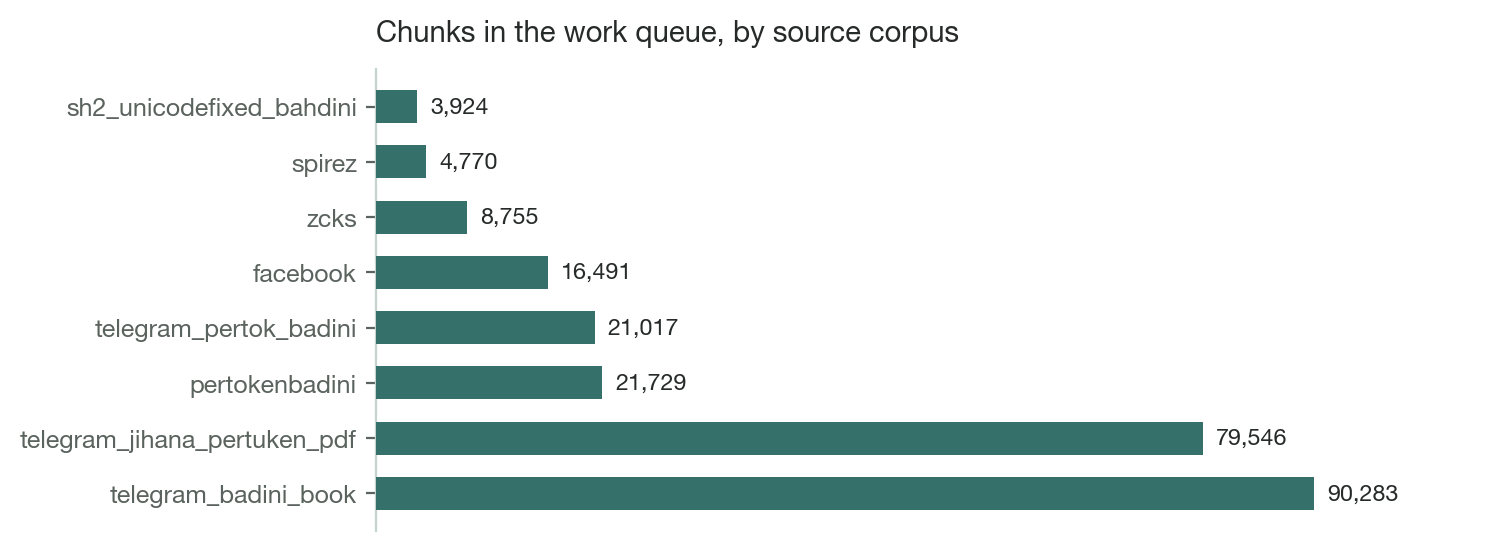
\includegraphics[width=0.94\textwidth]{fig_chunks_by_source.png}
\end{center}

By origin the queue splits 166,169 chunks from the reviewed OCR corpus against
80,346 from native extraction --- roughly two to one in favour of OCR, because
OCR reads the rendered page image and is therefore immune to the PDF font
problems that sent so many native extractions to the reject pile.

% ===========================================================================
\clearpage
\section{The pipeline end to end}

\begin{figure}[h]
\centering
\begin{tikzpicture}[node distance=6mm]
  \node[diagram node, text width=30mm] (queue) {chunks.jsonl\\{\footnotesize 246,515 chunks}};
  \node[diagram accent, right=10mm of queue, text width=32mm] (gen)
    {generate\_qa\_openrouter\\{\footnotesize 1 API call per chunk}};
  \node[diagram node, right=10mm of gen, text width=31mm] (recs)
    {generations/*.jsonl\\{\footnotesize 248,243 records}};
  \node[diagram accent, below=9mm of recs, text width=31mm] (comp)
    {compile\_qa\_dataset\\{\footnotesize adds context mode}};
  \node[diagram node, left=10mm of comp, text width=32mm] (out)
    {qa\_pairs.jsonl\\{\footnotesize 952,801 records}};
  \node[diagram node, left=10mm of out, text width=30mm] (exp)
    {csv · parquet · outliers\\{\footnotesize derived views}};

  \draw[diagram arrow] (queue) -- (gen);
  \draw[diagram arrow] (gen) -- (recs);
  \draw[diagram arrow] (recs) -- (comp);
  \draw[diagram arrow] (comp) -- (out);
  \draw[diagram arrow] (out) -- (exp);
  \draw[diagram arrow, dashed] (recs.north) .. controls +(0,7mm) and +(0,7mm) .. (gen.north)
    node[midway, above, font=\uifont\scriptsize, text=inksoft] {resume: skip ok/empty};
\end{tikzpicture}
\end{figure}

\vspace{-2mm}
The dashed edge is the resume path and is what made a four-day, restartable run
possible. Each processed chunk appends one record to a per-document file, and a
re-run reads those files first and skips anything already recorded as
\codeid{ok} or \codeid{empty}. Failures are deliberately \emph{not} recorded as
done, so they are retried automatically on the next run without a separate
pass.

% ===========================================================================
\section{Generation}

\subsection{The model, and why this one}

\begin{tabularx}{\textwidth}{@{}p{4.2cm}L@{}}
\tablehead{PARAMETER} & \tablehead{VALUE AND REASONING}\\
\midrule
Model & \codeid{google/gemini-3.1-flash-lite} via OpenRouter\\
Temperature & \codeid{0.7} --- four pairs are requested in a single call, and
lower temperatures made the four read as restatements of one another\\
Max output tokens & \codeid{2048} --- four Bahdini pairs with reasoning
average 605 output tokens, so this is headroom, not a target\\
Messages & \emph{one} \codeid{user} message. No system role is sent\\
Response format & none --- no JSON mode; the schema is enforced by the prompt
and validated after the fact\\
Request timeout & 180 seconds per attempt\\
Prompt version & \codeid{v3}, recorded on every output record\\
\bottomrule
\end{tabularx}

\vspace{0.6em}
The tier was chosen by pilot rather than by assumption. Forty chunks were run
at three pairs each and forty at four; \codeid{flash-lite} returned the full
requested count on 39 of 40 either way, and the fourth pair read as a genuinely
distinct question rather than filler. The stronger \codeid{pro} tier was
therefore not needed, and the difference is roughly a factor of five in cost.

\begin{warmcard}
{\uimed\fontsize{8.5}{11}\selectfont\color{crail}TWO PROMPTS, EASILY CONFUSED}\par\vspace{0.3em}
The configuration defines \codeid{QA\_GENERATION\_PROMPT\_TEMPLATE} and
\codeid{QA\_SYSTEM\_PROMPT}, and they are unrelated. The first is what Gemini
sees at generation time and never appears in the delivered dataset. The second
is what Gemma sees at fine-tuning time, written into the \codeid{system} slot
of finished records by the compile step, and never sent to Gemini. Editing the
wrong one changes nothing about what is generated, or everything about the
delivered records while leaving generation untouched.
\end{warmcard}

\subsection{The exact prompt}

Reproduce this at any time with
\codeid{python3 -c "import qa\_config as c; print(c.build\_qa\_prompt('<CHUNK>'))"}.
Rendered with \codeid{n\_pairs=4}, the complete user message is:

\begin{corpuscard}
{\footnotesize\ttfamily\setstretch{1.08}
You are building instruction-tuning data for a 100\% pure Bahdini (Badini)
Kurdish language model. Bahdini is spoken by people in Dohuk city and
governorate.\\[0.5em]
Below is one excerpt ("the context") from a Bahdini text. Write 4
question-answer pairs a person could ask about this excerpt, as if using it for
reading comprehension / instruction fine-tuning.\\[0.5em]
Rules:\\
- CRITICAL DIALECT RULE: Both the question and the answer MUST be written in
100\% pure Bahdini Kurdish (Arabic script) exactly as spoken in Dohuk. Do NOT
mix in any Sorani words, phrases, or grammar. Do NOT use general Kurmanji
vocabulary or Latin script. You must ensure the dialect is strictly pure
Bahdini.\\
- The answer must be grounded in the context: prefer extractive answers quoting
or closely paraphrasing the text; reasonable inference/synthesis is fine for
explanatory or summarization questions, but never introduce facts that are not
supported by the context.\\
- Do not ask about the excerpt's formatting, page numbers, or the fact that it
is an excerpt.\\
- Vary the question\_type across the set; choose only from: factual,
explanatory, summarization, definitional, inferential.\\
- If the context is too short, garbled, or content-free to support 4 distinct,
well-grounded questions, return fewer pairs (an empty list is fine) rather than
inventing filler.\\
- If answering the question genuinely requires connecting multiple details in
the context or drawing a conclusion beyond a single stated fact, also fill in
"reasoning": a brief step-by-step justification, in pure Bahdini Kurdish, for
how the answer follows from the context. If the question is directly answerable
by quoting or restating one explicit fact, set "reasoning" to null; do not pad
it with filler.\\[0.5em]
Output strict JSON only: a list of objects, no markdown fences, no commentary
before or after. Each object must have exactly these keys:\\
\hspace*{2em}"question": string\\
\hspace*{2em}"answer": string\\
\hspace*{2em}"question\_type": one of ['factual', 'explanatory', 'summarization',
'definitional', 'inferential']\\
\hspace*{2em}"reasoning": string or null (see rule above)\\[0.5em]
Context:\\
"""\\
\{context\}\\
"""}
\end{corpuscard}

Two details worth knowing before anyone edits this. First, the
\codeid{one of ['factual', ...]} line renders a raw Python list repr, quotes
included, because that value is interpolated directly while the bullet above it
is comma-joined. It is cosmetically untidy and the model complies with it
regardless --- but tidying it mid-corpus would mean a new prompt version, and a
version bump part-way through leaves the delivered dataset generated under two
different sets of instructions. Second, the shouty phrasing of the dialect rule
is deliberate: version v2 said only ``must be written in Bahdini Kurdish (do
not switch to Sorani, Latin-script Kurdish, or Arabic)'', and review found
Sorani and general-Kurmanji vocabulary leaking in anyway. Version v3 names the
three prohibitions separately and marks the rule critical.

\subsubsection{Prompt version history}

\begin{tabularx}{\textwidth}{@{}p{1.6cm}L@{}}
\tablehead{VERSION} & \tablehead{CHANGE}\\
\midrule
v1 & Initial. Three pairs per chunk, 700-token context target, no reasoning field.\\
v2 & Added the optional \codeid{reasoning} field, the 70/30 context split, and
the 900-token context target, after the partner confirmed the token budget
covers the prompt side only.\\
v3 & Current. Rewrote the dialect rule after Sorani leakage was observed;
reasoning must also be pure Bahdini. All 248,243 records on disk are v3.\\
\bottomrule
\end{tabularx}

\subsection{What the model returned}

\begin{center}
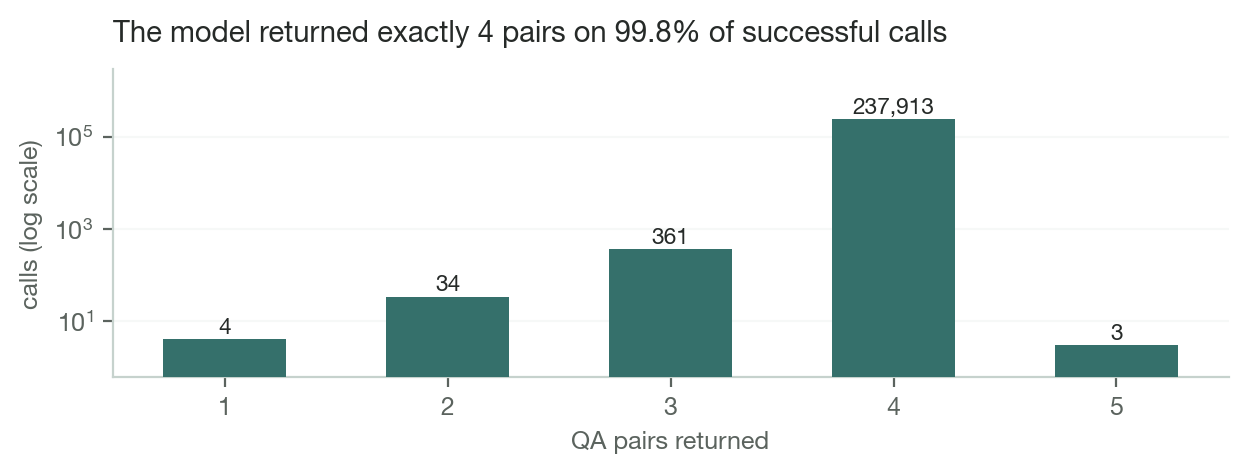
\includegraphics[width=0.94\textwidth]{fig_pairs_per_call.png}
\end{center}

\vspace{-2mm}
Of 238,315 successful calls, 237,913 returned exactly the four pairs requested
--- 99.83\%. The parser accepts a variable count by design, so the handful that
returned one, two, three or five pairs were kept rather than discarded. Five
pairs is possible because the parser validates structure, not cardinality.

\begin{tabularx}{\textwidth}{@{}p{2.9cm}rrL@{}}
\tablehead{STATUS} & \tablehead{CALLS} & \tablehead{SHARE} & \tablehead{MEANING AND RETRY BEHAVIOUR}\\
\midrule
\codeid{ok} & 238,315 & 95.99\% & at least one valid pair. Not retried\\
\codeid{empty} & 8,209 & 3.31\% & model returned \codeid{[]} --- the intended
answer for a garbled or content-free chunk. Not retried\\
\codeid{parse\_error} & 1,687 & 0.68\% & response was not a JSON list, or every
entry was malformed. \textbf{Retried automatically}\\
\codeid{error} & 32 & 0.01\% & HTTP or network failure after five attempts.
\textbf{Retried automatically}\\
\bottomrule
\end{tabularx}

\vspace{0.6em}
\kw{The empty responses are not failures.} They are the model correctly
declining to invent content for a chunk that cannot support four grounded
questions, which the prompt explicitly instructs it to do. Treating that 3.31\%
as a defect would mean asking for filler. What genuinely produced nothing is
\codeid{parse\_error} plus \codeid{error}: 1,719 chunks, 0.70\% of the queue.

\subsection{Failure handling}

Transport failures retry five times with exponential backoff plus jitter,
computed as $2 \cdot 2^{n} + \mathrm{rand}(0,1)$ seconds, on HTTP 429 and any
5xx. HTTP 402 and 403 are treated as terminal and are \emph{not} retried: they
mean credit exhausted or key rejected, and retrying them would burn five
backoff cycles per chunk against a dead key while the run appeared to be
working. Hitting either sets a stop flag that drains in-flight requests and
ends the run cleanly.

At the pair level, the parser strips any markdown fence, parses the JSON, and
keeps only entries with a non-empty question, a non-empty answer, and a
\codeid{question\_type} drawn from the five agreed values. A single malformed
pair inside an otherwise-valid response is dropped; it does not fail the chunk.

\begin{figure}[h]
\centering
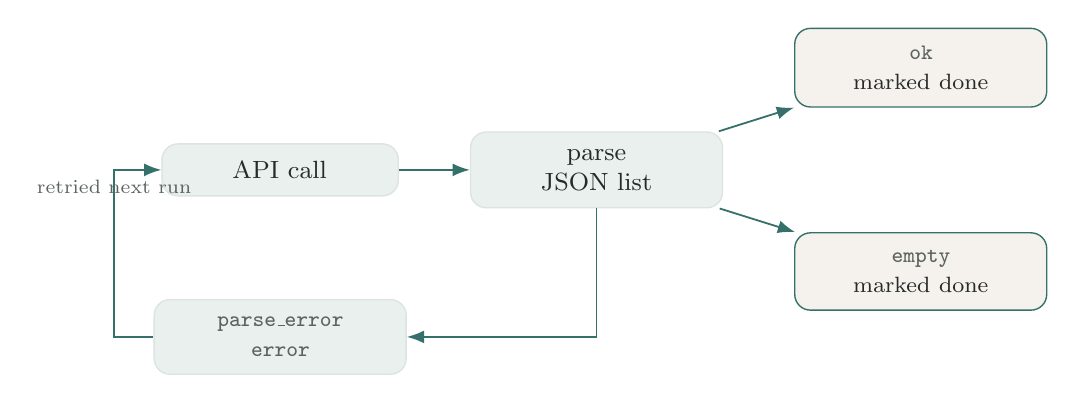
\begin{tikzpicture}[node distance=5mm]
  \node[diagram node, text width=24mm] (call) {API call};
  \node[diagram node, right=9mm of call, text width=26mm] (parse) {parse\\JSON list};
  \node[diagram accent, above right=3mm and 9mm of parse, text width=26mm] (ok) {\codeid{ok}\\{\footnotesize marked done}};
  \node[diagram accent, below right=3mm and 9mm of parse, text width=26mm] (empty) {\codeid{empty}\\{\footnotesize marked done}};
  \node[diagram node, below=13mm of call, text width=26mm] (fail) {\codeid{parse\_error}\\\codeid{error}};

  \draw[diagram arrow] (call) -- (parse);
  \draw[diagram arrow] (parse) -- (ok);
  \draw[diagram arrow] (parse) -- (empty);
  \draw[diagram arrow] (parse.south) |- (fail.east);
  \draw[diagram arrow] (fail.west) -| ($(call.west)+(-6mm,0)$) |- (call.west)
    node[pos=0.25, below, font=\uifont\scriptsize, text=inksoft] {retried next run};
\end{tikzpicture}
\end{figure}

\subsection{Throughput, concurrency and the overnight run}

The full corpus was generated across several sessions between 6 and 10 August
2026. Sustained throughput was roughly 450 chunks per minute at concurrency 32
with a dispatch batch of 128, up from about 230 per minute at concurrency 16.

Batch size matters more than it looks: the dispatcher waits for every request
in a batch before starting the next, so the batch is a barrier. Setting it at
or below the concurrency level starves the semaphore whenever a single slow
request holds up its batch, which is why 128 pairs with a concurrency of 32
rather than the default 16.

The unattended portion ran under a supervisor that restarts the generator if it
exits with work pending. That loop introduced one hazard worth recording: the
generator's budget cap is evaluated \emph{per run}, so a naive restart loop
would silently reset the cap on every iteration. The supervisor therefore reads
remaining credit back from the provider before each attempt and passes that,
minus a small reserve, as that attempt's cap --- so the ceiling tracks
cumulative spend across restarts, with the provider's own key limit as a hard
backstop underneath.

\subsection{Cost, and a bug that mattered}

\begin{tabularx}{\textwidth}{@{}Lrr@{}}
\tablehead{QUANTITY} & \tablehead{TOKENS} & \tablehead{RATE (USD/M)}\\
\midrule
Input (prompt) & 304,524,932 & 0.25\\
Output (completion) & 150,188,299 & 1.50\\
\midrule
Total billed & 454,713,231 & \\
\bottomrule
\end{tabularx}

\vspace{0.4em}
Mean consumption per call was 1,227 input and 605 output tokens. Total spend
was \kw{\$301.41}: \$0.316 per thousand pairs, or \$0.00122 per source chunk.

Pricing is keyed by exact model slug. It previously was not --- a single pair
of constants for the \codeid{pro} tier was applied to every run regardless of
which model was actually called, which overstated \codeid{flash-lite} runs by a
factor of 3.75. That was not merely a display error. \kw{The budget cap is
evaluated against this estimate}, so an inflated rate makes a run halt far
short of its real budget while appearing to have completed: the first
full-corpus attempt carried a \$350 cap and would have stopped at roughly 32\%
of the queue having actually spent about \$93.

\begin{sagecard}
{\uimed\fontsize{8.5}{11}\selectfont\color{crail}THE COST MODEL IS VALIDATED, NOT ASSUMED}\par\vspace{0.3em}
Recomputing every record on disk from its stored token counts gives \$50.04 for
the first API key; the provider's own usage endpoint reports \$50.0542 for the
same key. That is a 0.03\% discrepancy across 41,467 calls, which is why the
figures in this report are stated as measurements rather than estimates. An
unknown model slug deliberately falls back to the most expensive known rate, so
the failure mode is stopping early rather than overspending.
\end{sagecard}

% ===========================================================================
\clearpage
\section{From pairs to training records}

\subsection{How 246,515 chunks became 952,801 records}

\begin{figure}[h]
\centering
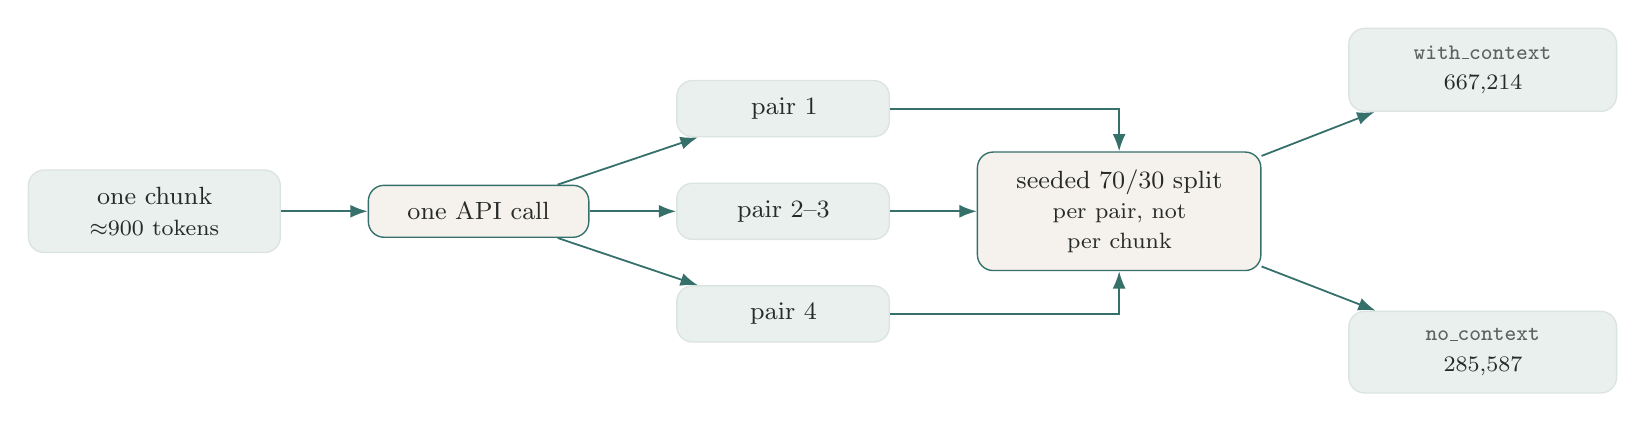
\begin{tikzpicture}[node distance=4mm]
  \node[diagram node, text width=26mm] (chunk) {one chunk\\{\footnotesize $\approx$900 tokens}};
  \node[diagram accent, right=11mm of chunk, text width=22mm] (call) {one API call};
  \node[diagram node, above right=6mm and 11mm of call, text width=21mm] (p1) {pair 1};
  \node[diagram node, right=11mm of call, text width=21mm] (p2) {pair 2--3};
  \node[diagram node, below right=6mm and 11mm of call, text width=21mm] (p4) {pair 4};
  \node[diagram accent, right=11mm of p2, text width=30mm] (split)
    {seeded 70/30 split\\{\footnotesize per pair, not per chunk}};
  \node[diagram node, above right=5mm and 11mm of split, text width=28mm] (wc)
    {\codeid{with\_context}\\{\footnotesize 667,214}};
  \node[diagram node, below right=5mm and 11mm of split, text width=28mm] (nc)
    {\codeid{no\_context}\\{\footnotesize 285,587}};

  \draw[diagram arrow] (chunk) -- (call);
  \draw[diagram arrow] (call) -- (p1);
  \draw[diagram arrow] (call) -- (p2);
  \draw[diagram arrow] (call) -- (p4);
  \draw[diagram arrow] (p1) -| (split);
  \draw[diagram arrow] (p2) -- (split);
  \draw[diagram arrow] (p4) -| (split);
  \draw[diagram arrow] (split) -- (wc);
  \draw[diagram arrow] (split) -- (nc);
\end{tikzpicture}
\end{figure}

\vspace{-2mm}
The context mode is assigned \emph{per pair} with a fixed seed, not per chunk.
That matters: assigning per chunk would mean all four pairs from a passage
share a mode, which correlates the split with document content. A fixed seed
makes the assignment reproducible across re-runs of the compile step over the
same generation records rather than reshuffled each time.

The delivered count is 952,801 rather than the 952,822 pairs on record. The
difference is 21 pairs referencing six chunk ids that no longer exist in the
queue, orphaned when the corpus was rebuilt after the character-corruption fix.
They are dropped rather than delivered without their grounding text.

\subsection{Record anatomy}

\begin{figure}[h]
\centering
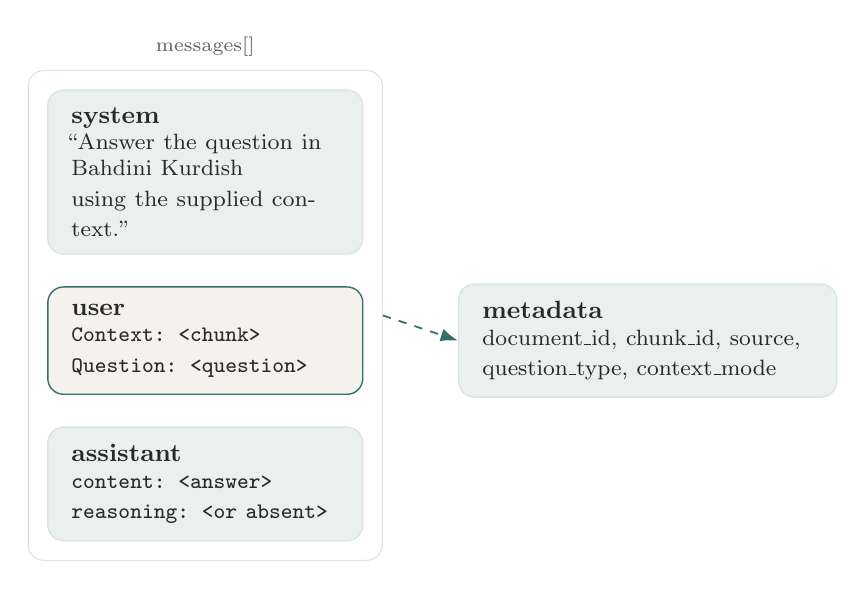
\begin{tikzpicture}[node distance=3mm]
  \node[diagram node, text width=34mm, align=left] (sys)
    {\textbf{system}\\{\footnotesize ``Answer the question in Bahdini Kurdish\\using the supplied context.''}};
  \node[diagram accent, below=4mm of sys, text width=34mm, align=left] (usr)
    {\textbf{user}\\{\footnotesize \texttt{Context: <chunk>}\\\texttt{Question: <question>}}};
  \node[diagram node, below=4mm of usr, text width=34mm, align=left] (asst)
    {\textbf{assistant}\\{\footnotesize \texttt{content: <answer>}\\\texttt{reasoning: <or absent>}}};
  \node[diagram node, right=12mm of usr, text width=42mm, align=left] (meta)
    {\textbf{metadata}\\{\footnotesize document\_id, chunk\_id, source,\\question\_type, context\_mode}};
  \node[fit=(sys)(asst), draw=creamline, rounded corners=2mm, inner sep=2.4mm] (msgbox) {};
  \node[above=0.5mm of msgbox, font=\uifont\scriptsize, text=inksoft] {messages[]};
  \draw[diagram arrow, dashed] (msgbox.east) -- (meta.west);
\end{tikzpicture}
\end{figure}

\vspace{-2mm}
For a \codeid{no\_context} record the user message is only
\codeid{Question: <question>}, and the system prompt switches to ``Answer the
question in Bahdini Kurdish'' --- dropping ``using the supplied context'',
which would be false when there is none. That second system string was a
judgement call rather than a specified requirement, and is a one-line change if
different wording is preferred.

\begin{warmcard}
{\uimed\fontsize{8.5}{11}\selectfont\color{crail}THE REASONING FIELD IS NATIVE, NOT INVENTED}\par\vspace{0.3em}
Gemma 4's own chat template reads \codeid{message.get('reasoning')} directly off
the assistant message and renders it into the model's thought channel ahead of
the answer. Verified directly against the template: passing
\codeid{reasoning} as a sibling key of \codeid{content} produces a
\codeid{<|channel>thought} block, whereas inlining a hand-rolled marker into
the content itself is treated as literal answer text. This is why reasoning
lives in its own field rather than being concatenated into the answer.
\end{warmcard}

% ===========================================================================
\section{The finished dataset}

\subsection{Size in tokens}

Every record was tokenized with the real \codeid{google/gemma-4-31B-it}
tokenizer. The chat template's own per-record overhead was measured at 18.68
tokens on a sample rather than assumed.

\begin{center}
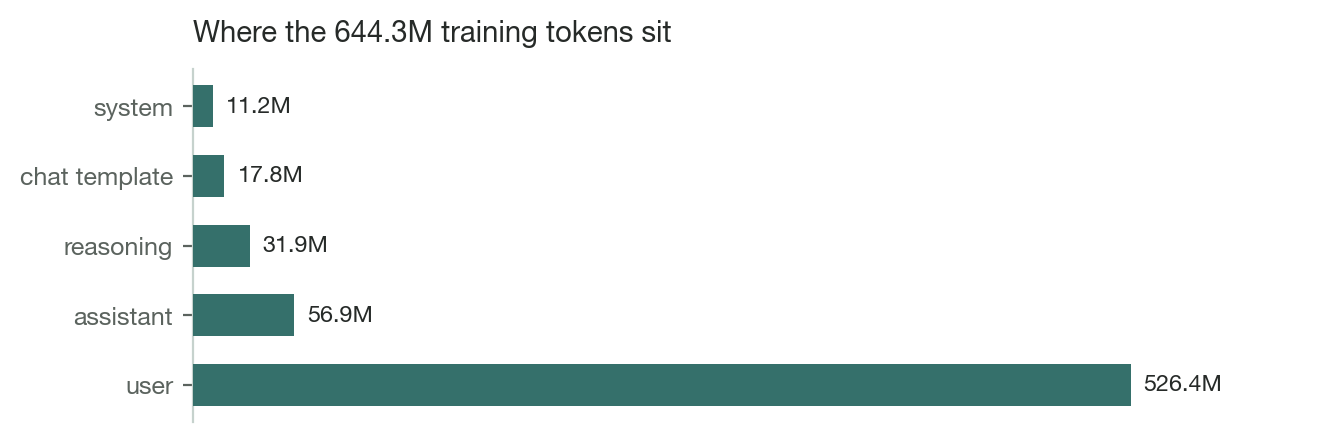
\includegraphics[width=0.94\textwidth]{fig_token_budget.png}
\end{center}

\begin{tabularx}{\textwidth}{@{}Lrr@{}}
\tablehead{COMPONENT} & \tablehead{TOKENS} & \tablehead{SHARE}\\
\midrule
User message (context + question) & 526,428,585 & 81.7\%\\
Assistant answer & 56,938,845 & 8.8\%\\
Reasoning & 31,896,635 & 5.0\%\\
Chat template overhead & 17,798,323 & 2.8\%\\
System prompt & 11,244,065 & 1.7\%\\
\midrule
\textbf{Total} & \textbf{644,306,453} & \textbf{100\%}\\
\bottomrule
\end{tabularx}

\vspace{0.6em}
The single most consequential number here is the first one. \kw{Context is
82\% of the training budget}, so any proposal to trim, filter or re-balance
context is a proposal about almost the entire dataset, while any change to
answers or reasoning touches at most a seventh of it.

\subsection{Length distribution}

\begin{center}
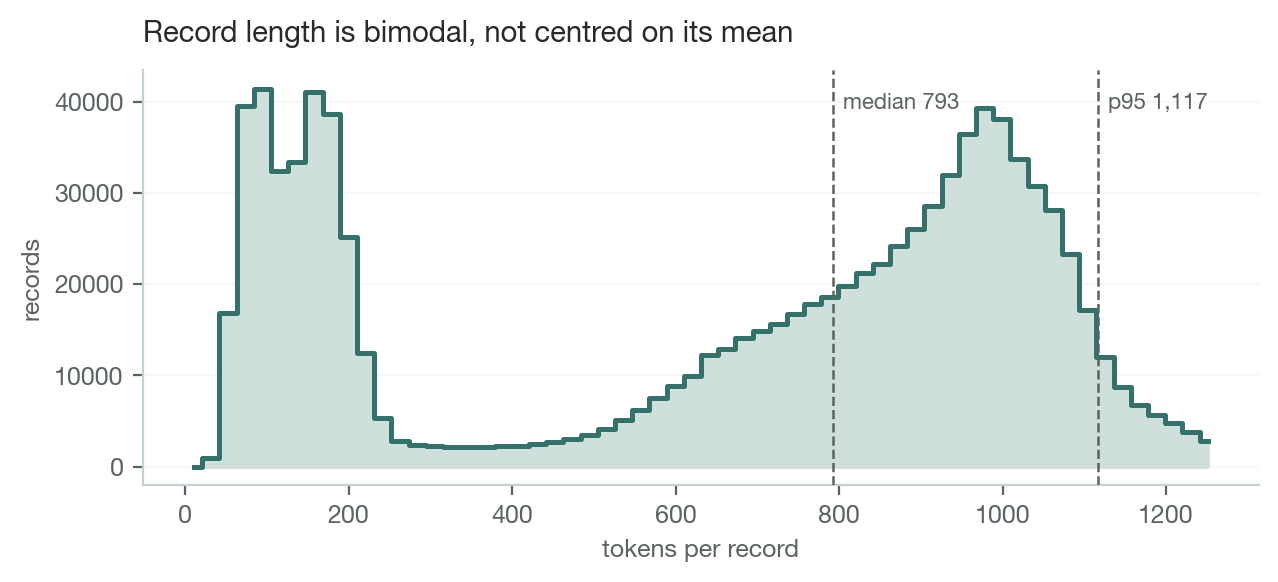
\includegraphics[width=0.94\textwidth]{fig_record_tokens.png}
\end{center}

\vspace{-2mm}
\kw{The mean is the wrong summary for this dataset.} Record length is bimodal:
bare-question records cluster near 90 tokens and context-carrying ones near
950, and the mean of 658 falls in the valley between them, describing almost no
actual record. The two populations should be reported --- and batched ---
separately.

\begin{tabularx}{\textwidth}{@{}Lrrrrrr@{}}
\tablehead{FIELD} & \tablehead{MIN} & \tablehead{P05} & \tablehead{MEDIAN} & \tablehead{MEAN} & \tablehead{P95} & \tablehead{MAX}\\
\midrule
User (prompt side) & 3 & 23 & 691 & 553 & 992 & 1,340\\
Assistant (answer) & 2 & 24 & 59 & 60 & 100 & 399\\
Whole record & 26 & 80 & 793 & 658 & 1,117 & 1,535\\
\bottomrule
\end{tabularx}

\vspace{0.6em}
Against the partner's roughly 1,000-token prompt-side mean, measured p95 is 992
and only 27 records in the entire corpus exceed the 1,300-token flag threshold
--- a 30\% allowance over the target. The budget was met comfortably.

\subsection{Context modes}

\begin{center}
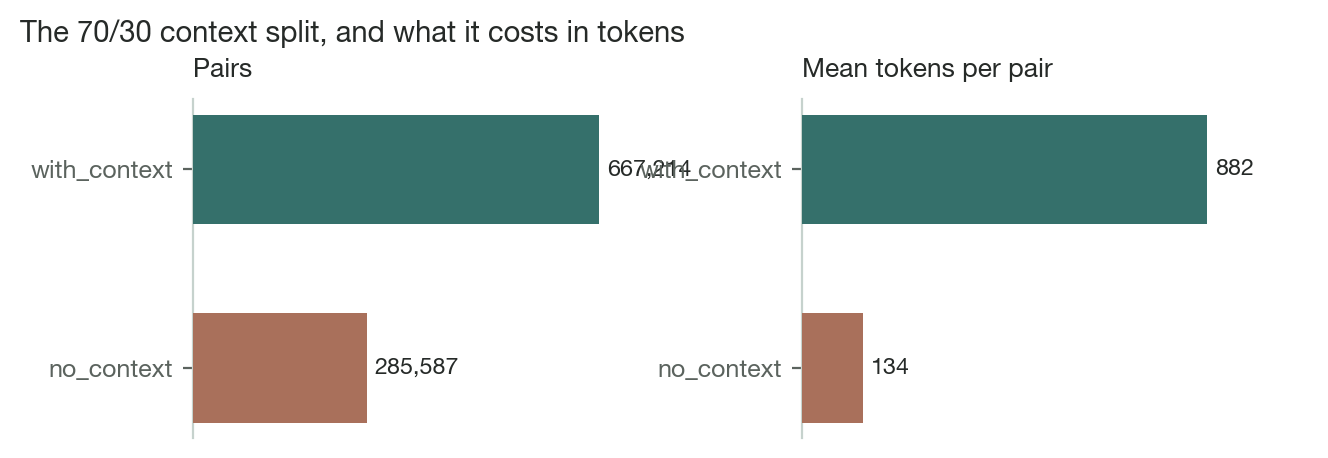
\includegraphics[width=0.94\textwidth]{fig_context_mode.png}
\end{center}

\vspace{-2mm}
The realised split is 667,214 \codeid{with\_context} against 285,587
\codeid{no\_context}: 70.03\% / 29.97\%, matching the configured ratio of 0.7
to two decimal places. The two modes exist because the model will be served
both ways --- retrieval-augmented and bare --- and a model trained only on
context-bearing prompts tends to refuse or hedge when the context is absent.
Both modes were generated with full context visible to the generator, so the
bare-question pairs remain grounded in real source text even though that text
is not shown at training time.

\subsection{Composition}

\begin{center}
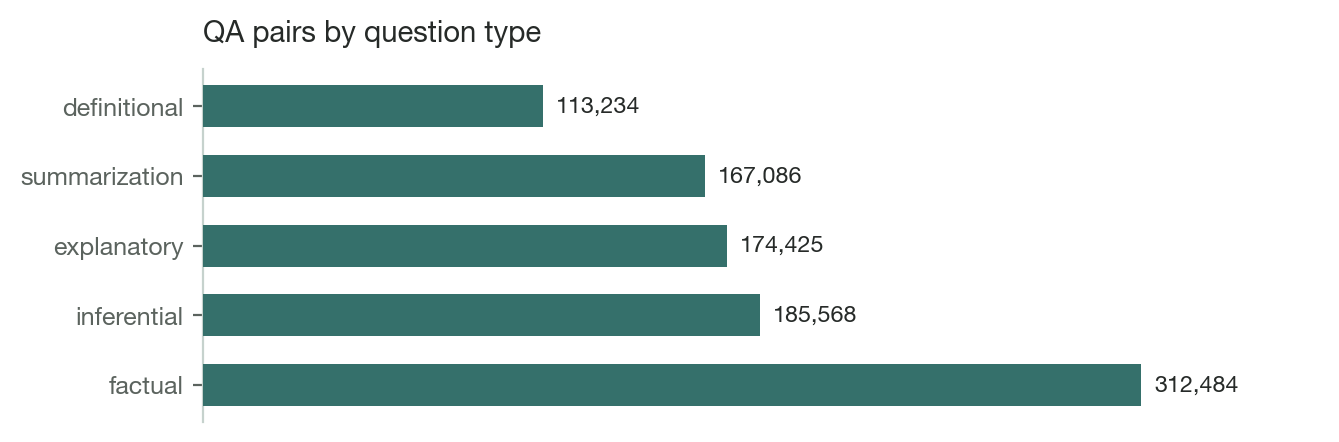
\includegraphics[width=0.94\textwidth]{fig_question_types.png}
\end{center}

\vspace{-1mm}
\begin{tabularx}{\textwidth}{@{}Lrr@{}}
\tablehead{SOURCE CORPUS} & \tablehead{PAIRS} & \tablehead{SHARE}\\
\midrule
telegram\_badini\_book & 350,085 & 36.7\%\\
telegram\_jihana\_pertuken\_pdf & 307,525 & 32.3\%\\
pertokenbadini & 85,524 & 9.0\%\\
telegram\_pertok\_badini & 81,012 & 8.5\%\\
facebook & 60,442 & 6.3\%\\
zcks & 33,971 & 3.6\%\\
spirez & 18,728 & 2.0\%\\
sh2\_unicodefixed\_bahdini & 15,514 & 1.6\%\\
\bottomrule
\end{tabularx}

\vspace{0.6em}
Two Telegram book collections are 69\% of the corpus. This reflects what
Bahdini text exists in bulk rather than any sampling decision, but it has a
direct consequence: \kw{any train/eval split must be stratified by source},
or the evaluation set measures those two collections and nothing else.

% ===========================================================================
\clearpage
\section{Quality findings}

Every anomaly found is collected in \codeid{qa\_outliers.csv}, one row per
flagged pair, keyed by \codeid{row\_index} back into the delivered file so any
decision maps to specific records. A pair can carry several flags.

\begin{center}
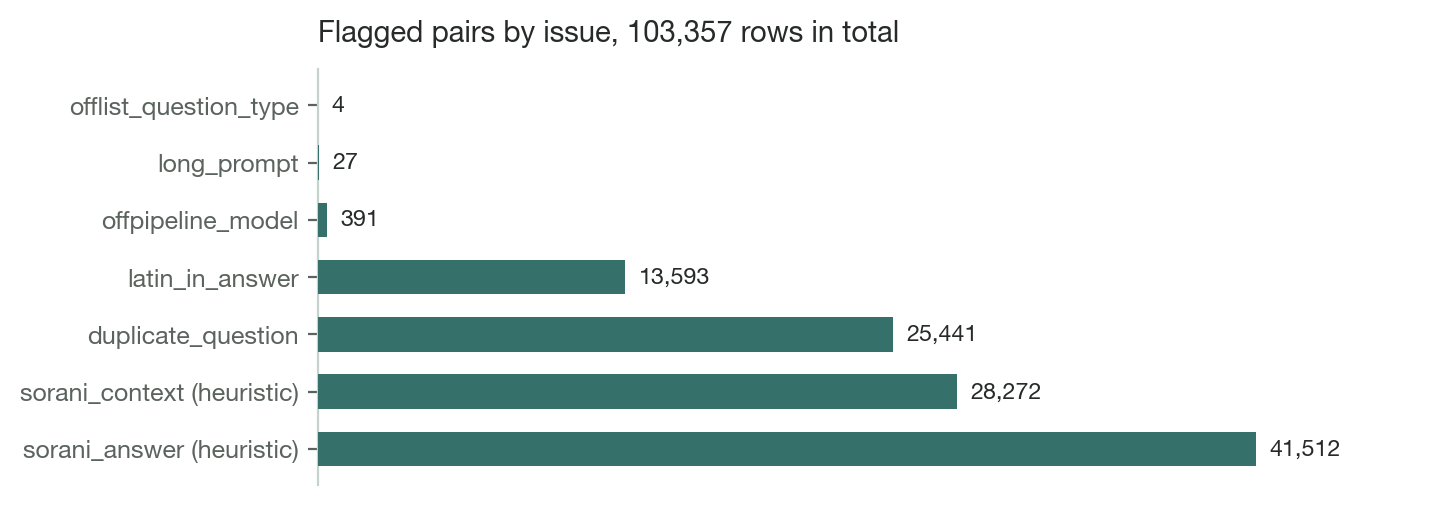
\includegraphics[width=0.94\textwidth]{fig_flags.png}
\end{center}

\begin{tabularx}{\textwidth}{@{}p{4.6cm}rL@{}}
\tablehead{FLAG} & \tablehead{ROWS} & \tablehead{NATURE}\\
\midrule
\codeid{sorani\_answer} & 41,512 & heuristic\\
\codeid{sorani\_context} & 28,272 & heuristic; the case that leaks into training\\
\codeid{duplicate\_question} & 25,441 & objective\\
\codeid{latin\_in\_answer} & 13,593 & objective; violates the prompt outright\\
\codeid{offpipeline\_model} & 391 & objective; from a one-off experiment\\
\codeid{long\_prompt} & 27 & objective; over the 1,300-token flag\\
\codeid{offlist\_question\_type} & 4 & objective\\
\midrule
\textbf{Total flagged rows} & \textbf{103,357} & 10.85\% of the dataset\\
\bottomrule
\end{tabularx}

\vspace{0.6em}
5,750 pairs carry two or more flags. Those are the highest-value rows to read
first, because independent signals agreeing is far stronger evidence than any
single heuristic firing alone.

\begin{warmcard}
{\uimed\fontsize{8.5}{11}\selectfont\color{crail}THE TWO DIALECT FLAGS ARE A QUEUE, NOT A VERDICT}\par\vspace{0.3em}
They come from a marker-frequency heuristic with no validated threshold, and
several of its markers occur in both dialects. The counts indicate how much
material is worth inspecting; they do not state how many rows are wrong. Both
\codeid{sorani\_score} and \codeid{bahdini\_score} are exposed as columns
precisely so the cutoff can be re-judged against real labels. Every other flag
in the table above is an objective, checkable property.
\end{warmcard}

\subsection{Sorani source text}

The most consequential finding. Some source chunks are Sorani rather than
Bahdini. The generator handles this correctly --- it obeys the dialect rule and
writes the question and answer in Bahdini regardless. The leak is at compile
time: for \codeid{with\_context} records the raw chunk is placed in the user
message, so Sorani text enters the training prompt of an otherwise-Bahdini
record.

\begin{corpuscard}
\corpusmeta{Sorani context found in the facebook corpus}{chunk text, excerpt}
\kurd{قەڵەمە پارکەرەکەی باوکم … بۆ وا بە کوڵ دەگریت؟}
\vspace{0.5em}

{\footnotesize\color{inksoft}Sorani orthography throughout --- the
\kurd{ەکەی} definite suffix and the \kurd{دەگریت} verb form are not Bahdini.
The question and answer generated from this chunk are correct Bahdini; the
context beneath them is not.}
\end{corpuscard}

\begin{center}
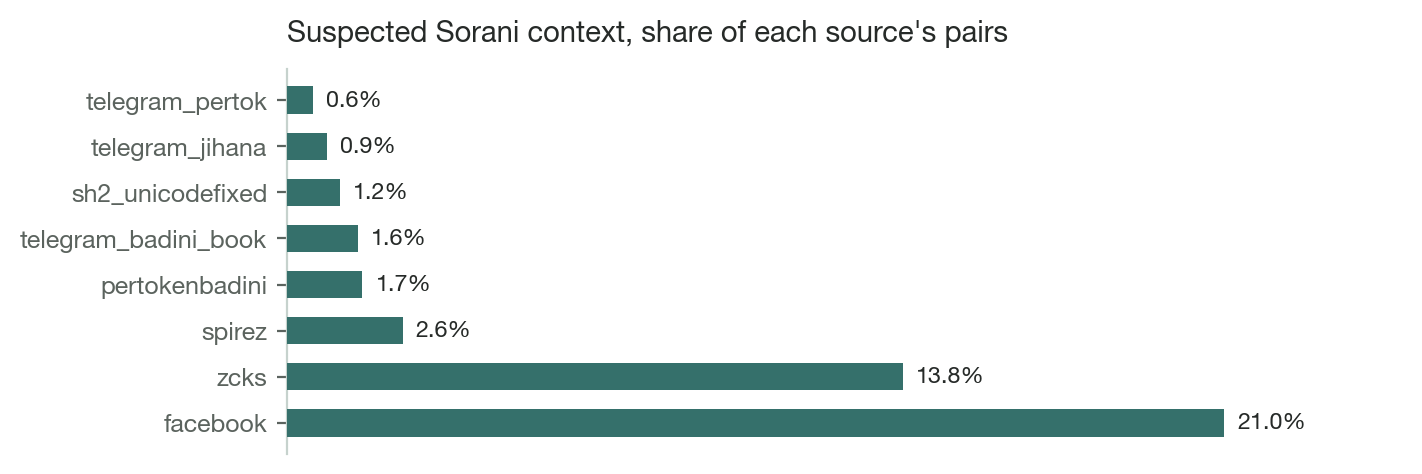
\includegraphics[width=0.94\textwidth]{fig_sorani_rate.png}
\end{center}

\vspace{-2mm}
Plotted as a rate rather than a count deliberately: by absolute count the large
Telegram corpora appear worst simply because they contain 350,000 pairs each.
Normalising shows the problem is concentrated in \codeid{facebook} (21.0\%) and
\codeid{zcks} (13.8\%), an order of magnitude above the book corpora --- which
is consistent with provenance, since those two are social posts and a
mixed-dialect website rather than curated Bahdini books. The same
concentration appeared in an independent estimate made on a 2,404-row
stratified sample when the corpus was only 17\% complete, which is weak
corroboration that the signal is real even though the threshold is not
calibrated.

\subsection{Latin-script leakage}

13,593 answers (1.43\%) contain at least one Latin character, against a prompt
that forbids Latin script outright. The rate was also 1.43\% when the corpus
was 17\% complete, so this is structural rather than an artefact of the later
run. The class is mixed: proper nouns and citations alongside genuine leakage.
The tail is unambiguous --- the worst single record carries 244 Latin
characters, which turn out to be Emily Dickinson's \emph{``I never saw a
moor''} sitting in the source text.

\subsection{Duplicate questions}

25,441 pairs (2.7\%) repeat a question string seen earlier.
\kw{Do not deduplicate on the question alone.} The repeats are dominated by
generic questions --- the kind askable of almost any passage --- which arise
independently across unrelated chunks and carry entirely different answers.
Global deduplication on the question string would delete legitimately distinct
training pairs. Deduplicate on the \codeid{(question, answer)} pair, or on
question within a document.

\subsection{Off-schema rows}

175 chunks, producing 391 pairs, were generated by a one-off manual experiment
using a different model outside this pipeline. They carry no token counts and
therefore contribute nothing to any cost figure in this report. They are also
the only source of the four off-list \codeid{question\_type} values in the
corpus (\codeid{descriptive} three times, \codeid{comparative} once), which the
pipeline's own parser would have rejected. The pairs are otherwise valid
Bahdini and were left in place; the compile step does not re-validate
\codeid{question\_type}, so filter there if strict schema conformance is
required.

% ===========================================================================
\section{Open decisions}

None of the following are settled. Each requires a Bahdini speaker's judgement,
and each has an inexpensive fix once decided.

\begin{enumerate}
\item \kw{Calibrate the dialect threshold.} Label a few hundred rows from the
\codeid{facebook} and \codeid{zcks} slice by eye, then set the cutoff against
those labels. Everything else on this list is cheaper than this, and none of it
is blocked by it.

\item \kw{Handle Sorani contexts.} The cheap fix is at compile time: force
affected pairs to \codeid{no\_context} rather than dropping them, which keeps
the Bahdini question and answer and discards only the Sorani prompt text. The
thorough fix is a per-document dialect gate in the chunking stage, applied the
same way as the existing corruption gate --- per document, because dialect is a
property of the document and a per-chunk cutoff would shred documents on
line-wrapping noise.

\item \kw{Triage Latin leakage.} Sort by \codeid{latin\_chars\_in\_answer}
descending. The tail is obviously wrong and the head is mostly proper nouns; a
threshold somewhere between will do once someone reads twenty rows.

\item \kw{Deduplicate carefully.} On \codeid{(question, answer)} or within a
document --- never on the question string globally.

\item \kw{Stratify the evaluation split by source}, or it will measure two
Telegram corpora and nothing else.

\item \kw{Decide on the 395 off-schema pairs.} Small enough to simply drop if
strict conformance matters.
\end{enumerate}

% ===========================================================================
\section{Artifacts and reproduction}

\begin{tabularx}{\textwidth}{@{}p{4.9cm}rL@{}}
\tablehead{FILE} & \tablehead{SIZE} & \tablehead{PURPOSE}\\
\midrule
\codeid{qa\_pairs.jsonl} & 2.4 GB & the deliverable, 952,801 records\\
\codeid{parquet/} (4 shards) & 350 MB & same rows, Hub-ready, verified identical\\
\codeid{qa\_pairs.csv} & 2.2 GB & same rows, spreadsheet encoding\\
\codeid{qa\_outliers.csv} & 251 MB & 103,357 flagged pairs, 8 flags\\
\codeid{stats.json} & 18 KB & token counts and distributions\\
\codeid{sample.jsonl} & 77 KB & 40 records, every type $\times$ mode combination\\
\bottomrule
\end{tabularx}

\vspace{0.6em}
The three encodings of the deliverable are not approximations of one another.
The table exporter reconstructs records from the written table and diffs them
against the source JSONL; the current result is 952,801 against 952,801 with
zero mismatches.

\subsubsection{Rebuilding from scratch}

\begin{softcard}
{\footnotesize\ttfamily
python3 qa\_generation/pipeline/build\_chunks.py\\
python3 qa\_generation/pipeline/generate\_qa\_openrouter.py --concurrency 32 --batch-size 128\\
python3 qa\_generation/pipeline/compile\_qa\_dataset.py --sample-size 40\\
python3 qa\_generation/export/compute\_dataset\_stats.py\\
python3 qa\_generation/export/export\_dataset\_table.py --verify\\
python3 qa\_generation/export/export\_outliers.py}
\end{softcard}

Re-running the generator is always safe and always makes progress: completed
chunks are skipped, failures are re-attempted, and interruption at any point
loses nothing because every finished chunk is already flushed to disk.

\vspace{2mm}
\begin{center}
{\uifont\fontsize{7.5}{10}\selectfont\color{inksoft}%
Figures generated from \codeid{stats.json} and \codeid{qa\_outliers.csv}.
Token counts from \codeid{google/gemma-4-31B-it}.}\\[1mm]
\preparedby
\end{center}

\end{document}
